%%%
%
% $Autor: Wings $
% $Datum: 2023-06-05 $
% $Dateiname: IMU $
% $Version: 1 $
%
%%%


\chapter{Inertial Measurement Unit}  \label{chap:InertialMeasurementUnit}


\section{Introduction}

An Inertial Measurement Unit (IMU) is an electronic device that measures and reports a body's specific force, angular rate, and sometimes the orientation of the body. It consists of a combination of three sensors accelerometers,  gyroscopes, and magnetometer that work together to provide information about an object's acceleration, velocity, orientation, and gravitational forces.\cite{sabatini:2011}



Arduino's library \PYTHON{Arduino\_LSM9DS1} of the LSM9DS1 sensor contains three examples that allow the user to use one of the sensors with little effort. \Mynote{missing citation}

\begin{figure}[H]
    \centering
    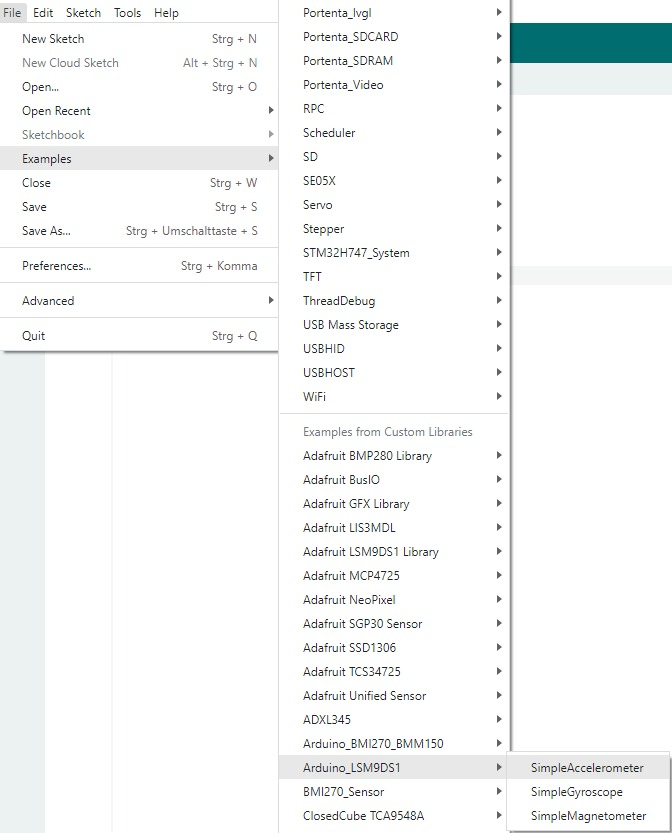
\includegraphics[width=0.7\textwidth]{IMU/LSM9DS1Bibliothek}
    \caption{Examples in the library \PYTHON{Arduino\_LSM9DS1}}
\end{figure}



\bigskip

In addition to accelerometers and gyroscopes, IMUs may also include magnetometers, which measure the direction and strength of magnetic fields. These sensors can help provide additional information about the orientation and movement of an object in relation to Earth's magnetic field.\cite{Wang:2022}

\bigskip

Inertial Measurement Units (IMUs) are commonly used in various fields such as aerospace, robotics, and gaming. The device is made up of multiple sensors that can measure the acceleration and angular rate of an object in three dimensions. The accelerometers measure linear motion in three axes (x, y, z), while the gyroscopes measure angular motion around these same axes.\cite{wahyudi:2011}


\section{6-Axis IMU LSM6DSOX}

The LSM6DSOX is a 6-axis IMU developed by STMicroelectronics that features a high-performance 3-axis digital accelerometer and 3-axis digital gyroscope. The device is designed for accurate motion tracking and is commonly used in applications such as wearable devices and smart phones. It can measure linear and rotational motion simultaneously.\cite{STMicroelectronics:2018} The device also includes a variety of other features such as a programmable digital signal processor (DSP), a configurable low-pass filter, and a built-in temperature sensor.

\bigskip

\section{IMU LSM6DSOX Features}

Features of the LSM6DSOX IMU, see \cite{STMicroelectronics:2018}, typically referring to the technical specifications and capabilities of the sensor.

\bigskip

 Here are the features of LSM6DSOX IMU features:

\begin{itemize}
\item  \textbf{Power consumption: }

      Power consumption is an important factor when it comes to battery-powered devices like nicla vision and smart phones. These devices are designed to be portable and convenient, and they rely on batteries to power them. Therefore, the power consumption of each component is a critical consideration to extend battery life and to provide better user experience.

     \bigskip
 
      The LSM6DSOX has a power consumption of 0.55 mA in combo high-performance mode. This means that the sensor can operate at a low power consumption level while still delivering high-performance data. In this mode, the sensor can measure both acceleration and angular rate simultaneously, and provide accurate and reliable data with a high sampling rate.
     
     \bigskip
     
      The combo high-performance mode is an optimized mode that reduces power consumption without compromising on data accuracy and reliability. It achieves this by using advanced algorithms and signal processing techniques to filter out noise and unwanted signals, resulting in high-quality data with low power consumption.
 

\item  \textbf{Always-on:}

 This means that the LSM6DSOX can be kept running all the time, even when a device is in sleep mode, without using up too much power. This is useful for applications that require continuous motion tracking, such as fitness tracking or navigation.


\item  \textbf{Smart FIFO: }

  The Smart FIFO (First In First Out)  is a buffer that can store up to 9 kilobytes of motion data. It is "smart" because it can be configured to store only the most important data, saving memory and reducing power consumption.\cite{Martinez:2022}


\item  \textbf{Android compatiblity:}
 
  The LSM6DSOX is compatible with the Android operating system, which is used in many smartphones and tablets.
 

\item  \textbf{Accelerometer full scale: }

 The accelerometer in the LSM6DSOX can detect motion in up to four different full-scale ranges, from ±2g to ±16g. full scale refers to the maximum range of acceleration that can be measured by the sensor without saturating or clipping the output signal. 

\bigskip

 For example, if an accelerometer has a full scale range of ±2g,\cite{Liu:2022} it means that the sensor can accurately measure accelerations up to 2g in both the positive and negative directions. If the measured acceleration exceeds this range, the sensor output will saturate at the maximum value, which may cause distortion in the output signal.

\item  \textbf{Gyroscope full scale: }
 
 The gyroscope in the LSM6DSOX can detect rotation in up to five different full-scale ranges, from ±125 degrees per second (dps) to ±2000 dps. Each range corresponds to a certain maximum angular velocity that the sensor can detect.

\item  \textbf{Analog supply voltage: }

 1.71 V to 3.6 V: This is the voltage range that the LSM6DSOX can operate at.

 \item  \textbf{Independent IO supply: }
 
 The input/output connections on the LSM6DSOX can operate at a separate voltage of 1.62 V.

 \item  \textbf{Compact footprint: }
 
 2.5 mm x 3 mm x 0.83 mm: This is the size of the LSM6DSOX package, which is small enough to fit many types of electronic devices.
 

\item  \textbf{SPI / I²C \& MIPI I3CSM serial interface with main processor data synchronization:}
 
 These are three different types of communication interfaces that the LSM6DSOX supports. The main processor data synchronization means that the data collected by the sensor can be synchronized with other sensors or data sources.


\item  \textbf{Auxiliary SPI for OIS data output for gyroscope and accelerometer: }
 
 This is an additional interface that can be used to output data from the gyroscope and accelerometer.

\item  \textbf{OIS configurable from Aux SPI, primary interface (SPI/I²C \& MIPI I3CSM): }
 
 The OIS (optical image stabilization) feature of the LSM6DSOX can be configured using either the auxiliary SPI or one of the other serial interfaces.

\item  \textbf{Advanced pedometer, step detector, and step counter: }
 
 These features allow the LSM6DSOX to accurately track the number of steps taken by a person wearing a device that contains the sensor.

\item  \textbf{Significant Motion Detection, Tilt detection: }
 
 The LSM6DSOX can detect significant motion events, such as a sudden acceleration or deceleration, as well as changes in orientation or tilt.

\item  \textbf{Standard interrupts:}
 
 Free-fall, wakeup, 6D/4D orientation, click and double-click: These are pre-programmed events that can trigger.
 
\end{itemize}

\section{IMU LSM6DSOX Data}

The LSM6DSOX is a type of Inertial Measurement Unit (IMU) sensor that measures acceleration, angular speed and temperature. The data output from this sensor includes acceleration, gyroscope, and temperature measurements.

\bigskip

 Accelerometer that measures the acceleration (Ax, Ay, Az) the rate of change of acceleration over time. The acceleration in each axis is typically reported in units of meters per second squared ($m/s^2$). For example, if the LSM6DSOX measures an acceleration of 5 $m/s^2$ in the x-axis, it means that the object being measured is increasing in velocity by 5 meters per second every second in the x-direction. See figure \ref{fig: Axis Acceleration of Accelerometer Sensor}

\bigskip

 Gyroscope that measures the angular speed ($\Omega$x, $\Omega$y, $\Omega$z) is a measure of the rate of change of the orientation of the object being measured with respect to each axis. The angular velocity in each axis is typically reported in units of degrees per second ($^\circ/s$). For example, if the LSM6DSOX measures an angular velocity of 100$^\circ/s$ in the z-axis, it means that the object being measured is rotating at a rate of 100 degrees per second around the z-axis. See figure \ref{fig: Angular Speed of Gyroscope Sensor.PNG}

\bigskip

 Temperature sensor that measures the ambient temperature (T) in degrees celsius (°C). The temperature sensor is located on the same chip as the accelerometer and gyroscope, and it operates by detecting changes in the voltage output of a diode that is sensitive to temperature. The temperature sensor can be used in a variety of applications, such as monitoring the temperature of electronic devices, measuring the temperature of an environment in which the sensor is placed, or compensating for temperature changes in the output of the accelerometer and gyroscope.

\bigskip

\subsection{Accelerometer:}\cite{Chiang:2006}

\begin{figure}[h]
	\centering
	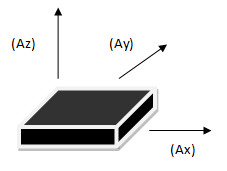
\includegraphics[width=6cm, height=5cm]{NiclaVision/SlopeControl/AxisAccelerationofAccelerometerSensor.PNG}
	\caption{\emph{Axis Acceleration of Accelerometer Sensor}}
	\label{fig: Axis Acceleration of Accelerometer Sensor}\Mynote{tikz!}
\end{figure}

\begin{itemize}
    \item Acceleration in X-axis (Ax): meters per second squared ($m/s^2$)
    \item Acceleration in Y-axis (Ay): meters per second squared ($m/s^2$)
    \item Acceleration in Z-axis (Az): meters per second squared ($m/s^2$)
\end{itemize}


\subsection{Gyroscope}

\begin{figure}[h]
	\centering
	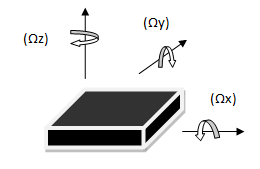
\includegraphics[width=6cm, height=5cm]{NiclaVision/SlopeControl/AngularSpeedofGyroscopeSensor.PNG}
	\caption{\emph{Angular Speed of Gyroscope Sensor}}
	\label{fig: Angular Speed of Gyroscope Sensor.PNG}
\end{figure}

\begin{itemize}
    \item Angular speed in X-axis (Roll, $\Omega$x): degrees per second ($^\circ/s$)
    \item Angular speed in Y-axis (Pitch, $\Omega$y): degrees per second ($^\circ/s$)
    \item Angular speed in Z-axis (Yaw, $\Omega$z): degrees per second ($^\circ/s$)
\end{itemize}

\section{Library setup in Arduino IDE}

Install the LSM6DSOX Library:

\begin{itemize}
	\item In the Arduino IDE, go to "Sketch" > "Include Library" > "Manage Libraries...".
	\item The Library Manager will open, providing a search bar.
	Type "LSM6DSOX" into the search bar.
	Look for the library called "LSM6DSOX" in the search results.
	\item Click on the library and then click the "Install" button to install the library.
\end{itemize}
\begin{figure}[h!]
	\centering
	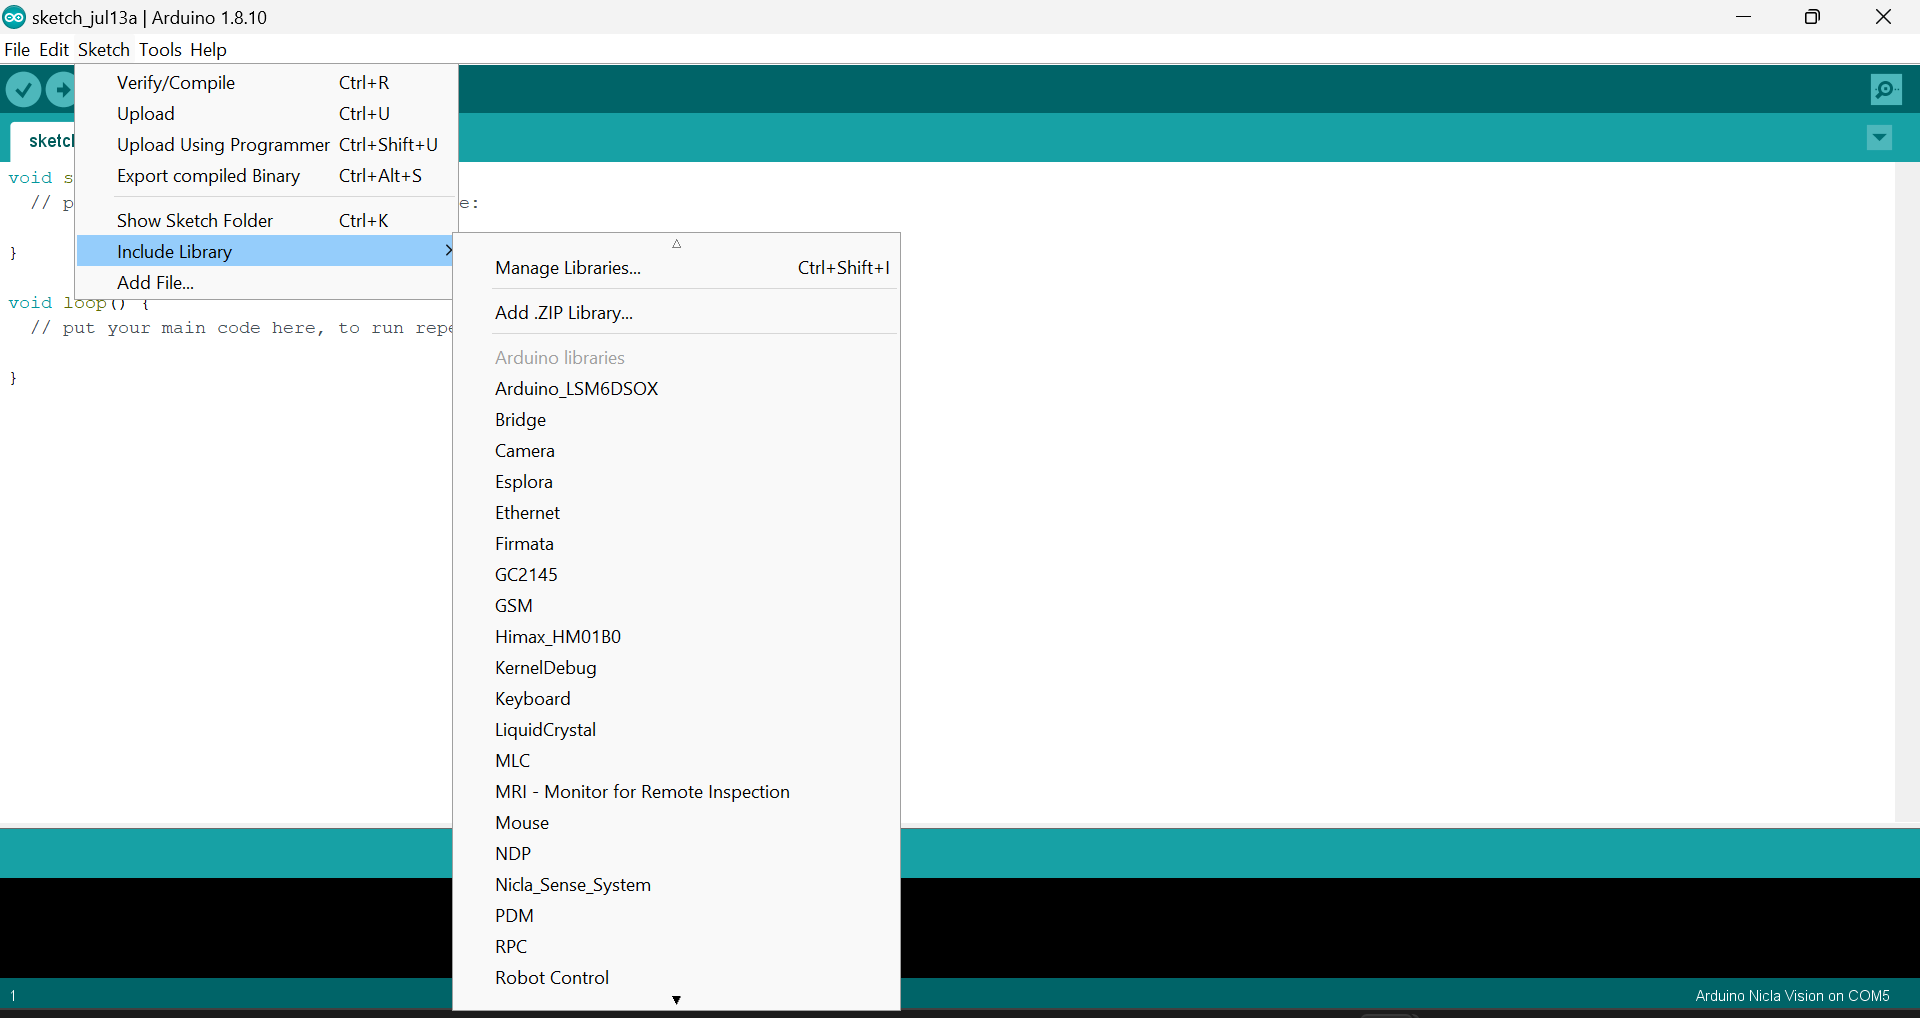
\includegraphics[width=12cm]{NiclaVision/SlopeControl/LibrarySetup.png}
	\caption{Library setup in Arduino IDE}
\end{figure}


\section{Applications}

 The LSM6DSOX 6-axis IMU (Inertial Measurement Unit) is a versatile sensor that combines a 3-axis accelerometer and a 3-axis gyroscope.

\begin{enumerate}
    \item \textbf{Motion tracking and gesture detection:} The LSM6DSOX IMU can be used to track the motion of a device and detect gestures such as shaking, tilting, and rotating. This application is particularly useful in gaming, virtual reality, and augmented reality applications.

    \item \textbf{Sensor hub:} The LSM6DSOX IMU can act as a sensor hub, collecting data from other sensors such as magnetometers, barometers, and GPS sensors. This enables the sensor to provide a more complete picture of the device's orientation and motion.\cite{Stefanicka:2017}

    \item \textbf{Indoor navigation:} The LSM6DSOX IMU can be used for indoor navigation by tracking the device's motion and orientation. This application is useful in navigation and location-based services in indoor environments where GPS signals are not available.

    \item \textbf{IoT and connected devices:} The LSM6DSOX IMU is an ideal sensor for IoT (Internet of Things) and connected devices. It can provide motion tracking data to a wide range of devices, such as smart homes, wearables, and industrial IoT devices.\cite{Tripathy:2022}

    \item \textbf{Smart power saving for handheld devices:} The LSM6DSOX IMU can be used to optimize power consumption in handheld devices by detecting when the device is idle or in motion. This information can be used to adjust the device's power settings and conserve battery life.

    \item \textbf{EIS and OIS for camera applications:} The LSM6DSOX IMU can be used to provide electronic image stabilization (EIS) and optical image stabilization (OIS) in camera applications. This allows for smoother video and reduces camera shake and blurring.

    \item \textbf{Vibration monitoring and compensation:} The LSM6DSOX IMU can be used to monitor vibration levels in machinery and compensate for the effects of vibration. This is useful in industrial applications where vibration can cause damage or reduce the performance of machinery.
\end{enumerate}


\section{LSM9DS1(IMU)}

\section{Features}

\begin{itemize}
    \item 3 acceleration channels, 3 angular rate channels, 3 magnetic field channels.
    \item ±2/±4/±8/±16 g linear acceleration full scale.
    \item ±4/±8/±12/±16 gauss magnetic full scale.
    \item ±245/±500/±2000 dps angular rate full scale.
    \item 16-bit data output.
\end{itemize}

\subsubsection{Applications}
\begin{itemize}
    \item Indoor navigation.
    \item Smart user interfaces.
    \item Advanced gesture recognition.
    \item Gaming and virtual reality input devices.
    \item Display/map orientation and browsing.
\end{itemize}

\subsubsection{Description}
The LSM9DS1 is a system-in-package featuring a 
3D digital linear acceleration sensor, a 3D digital angular rate sensor, and a 3D digital magnetic sensor.


\section{Pin description LSM9DS1}

\section{Pin connections LSM9DS1}

\begin{figure}[h!]
    \centering	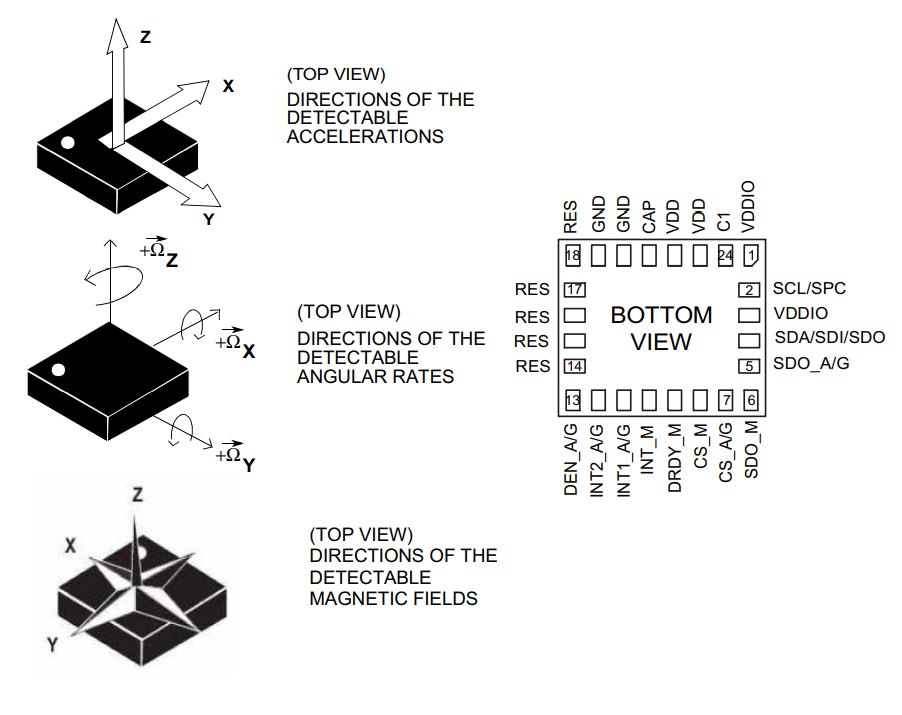
\includegraphics[width=\linewidth]{Nano33BLESense/imupin}
    \caption{\textbf{Pin connections LSM9DS1}} \cite{STMicroelectronics:2015}
\end{figure}


\subsubsection{Pin description LSM9DS1}
\begin{figure}[h!]
    \centering	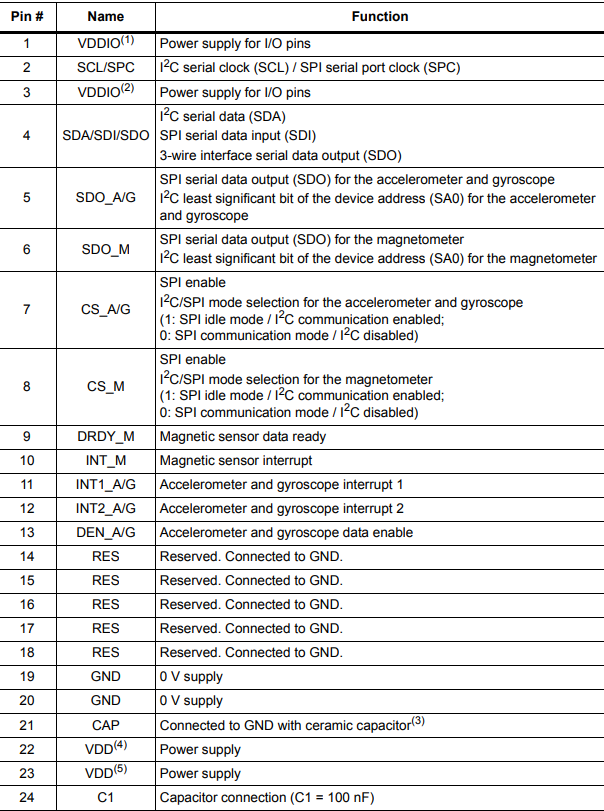
\includegraphics[width=14cm]{Nano33BLESense/imupin1}
    \caption{\textbf{Pin description LSM9DS1}} \cite{STMicroelectronics:2015}
\end{figure}

\subsection{Module specifications}
\subsubsection{Sensor characteristics}
\begin{figure}[h!]
    \centering	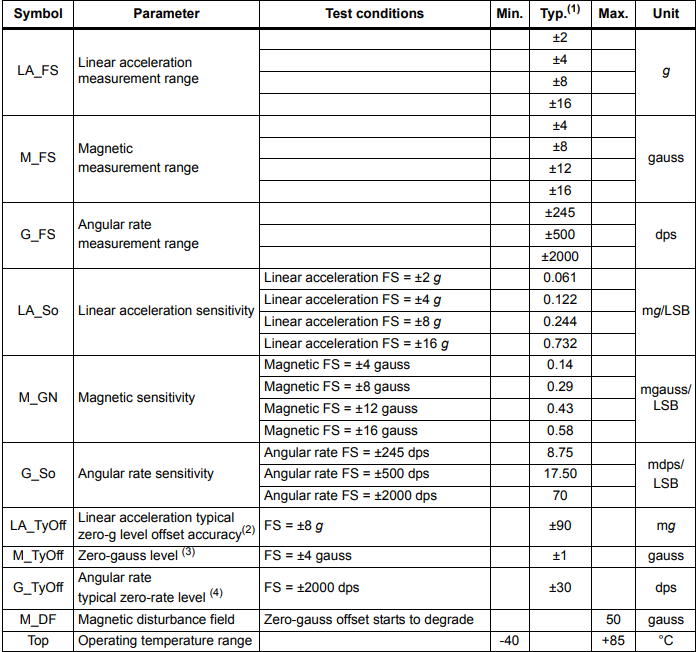
\includegraphics[width=\linewidth]{Nano33BLESense/sensorchara}
    \caption{\textbf{Sensor Characteristics}} \cite{STMicroelectronics:2015}
\end{figure}


\subsubsection{Temperature Sensor characteristics}
\begin{figure}[h!]
    \centering	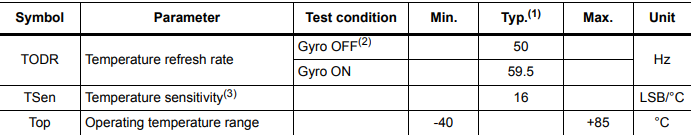
\includegraphics[width=\linewidth]{Nano33BLESense/tempchara}
    \caption{\textbf{Temperature Sensor Characteristics}} \cite{STMicroelectronics:2015}
\end{figure}

\subsubsection{Absolute Maximum Ratings}
Stresses above those listed as “Absolute maximum ratings” may cause permanent damage 
to the device. This is a stress rating only and functional operation of the device under these 
conditions is not implied. Exposure to maximum rating conditions for extended periods may 
affect device reliability

\begin{figure}[h!]
    \centering	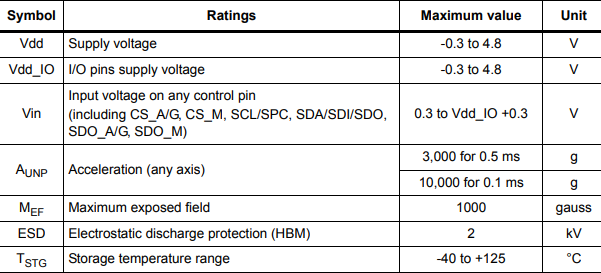
\includegraphics[width=\linewidth]{Nano33BLESense/absolmax}
    \caption{\textbf{Absolute Maximum Temperature }} \cite{STMicroelectronics:2015}
\end{figure}

\subsection{Block Diagram}

\subsubsection{Accelerometer and gyroscope digital block diagram}
\begin{figure}[h!]
    \centering	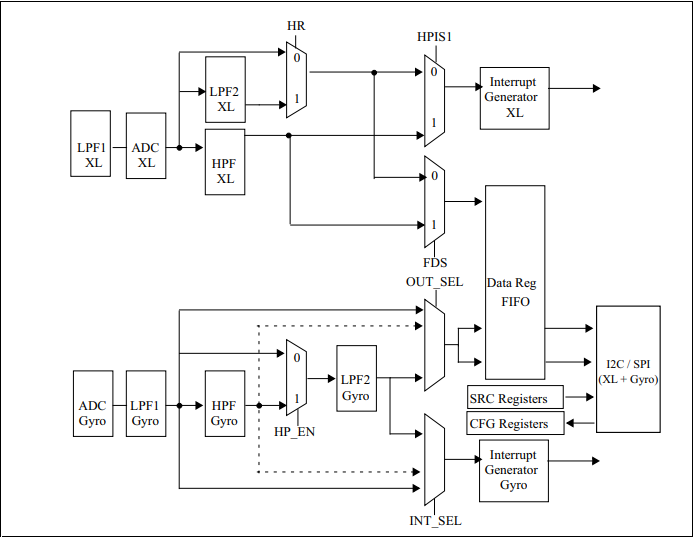
\includegraphics[width=\linewidth]{Nano33BLESense/acceandgyroblock}
    \caption{\textbf{Accelerometer and gyroscope block diagram}} \cite{STMicroelectronics:2015}
\end{figure}

\newpage
\subsubsection{Magnetometer digital block diagram}
\begin{figure}[h!]
    \centering	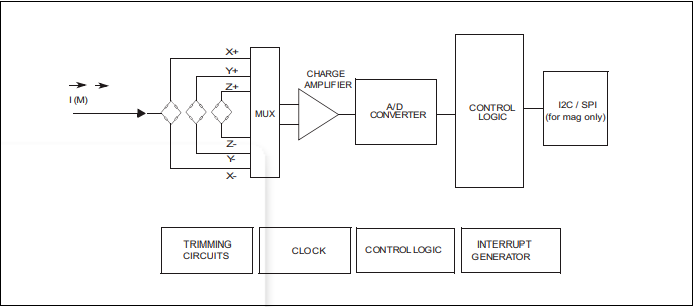
\includegraphics[width=\linewidth]{Nano33BLESense/magnetometerblock}
    \caption{\textbf{Magnetometer block diagram}} \cite{STMicroelectronics:2015}
\end{figure}

\newpage
\subsubsection{LSM9DS1 electrical connections}

\begin{figure}[h!]
    \centering	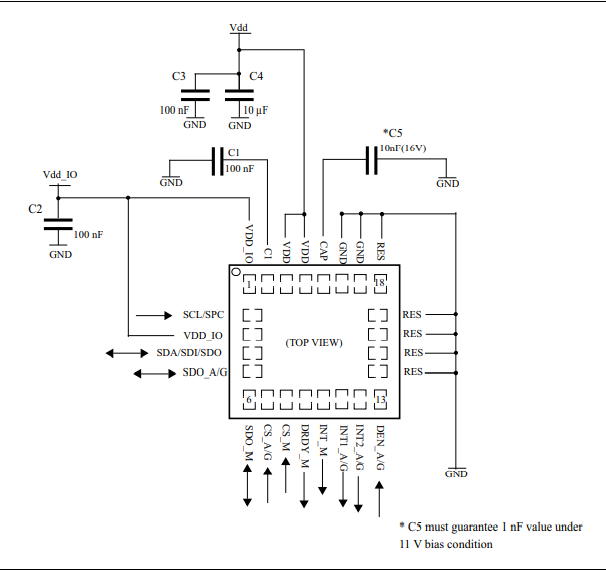
\includegraphics[width=\linewidth]{Nano33BLESense/elecon}
    \caption{\textbf{LSM9DS1 electrical connections}} \cite{STMicroelectronics:2015}
\end{figure}


\subsection{System Requirements}

\fcolorbox{blue}{blue!10}{\begin{minipage}{\textwidth}
        \begin{center}
            \begin{tabular}{llm{90mm}} 
                %\multicolumn{3}{l}{\large \textcolor{blue}{ Tech Specs of Arduino Nano 33 BLE Sense}} \\ \hline
                \\ \textbf{\MapleCommand{\textcolor{blue}{Operating System}}}  & Windows 7 or above, MacOS X or higher \\
                \textbf{\MapleCommand{\textcolor{blue}{CPU}}}  & Intel i3 or above\\
                \textbf{\MapleCommand{\textcolor{blue}{RAM}}}  & Min 2GB\\
                \textbf{\MapleCommand{\textcolor{blue}{Arduino IDE}}}  & V. 1.1819 \\
                \textbf{\MapleCommand{\textcolor{blue}{Boards}}}  & Arduino mBED OS Nano \\
                \textbf{\MapleCommand{\textcolor{blue}{Libraries}}}  & LSM9DS1 \\
                \textbf{\MapleCommand{\textcolor{blue}{Interface}}}  & USB port \\			
            \end{tabular}
        \end{center}
\end{minipage}}

\subsection{Precautions to be taken}

\begin{itemize}
    
    \item This equipment complies with RF radiation exposure limits set forth for an uncontrolled environment.
    \item This Transmitter must not be co-located or operating in conjunction with any other antenna or transmitter.
    \item The operating temperature of the EUT can't exceed 85$^{0}$C and shouldn't be lower than -40$^{0}$C.
    \item The Frequency band should be in between 863-870Mhz.
    \item Arduino Nano 33 BLE only supports 3.3V I/Os and is NOT 5V tolerant so please make sure you are not directly connecting 5V signals to this board or it will be damaged.
    \item Keep away from water or fire.
    \item Hold it gently, do not harm the components and sensors present on the board.
    
\end{itemize}

